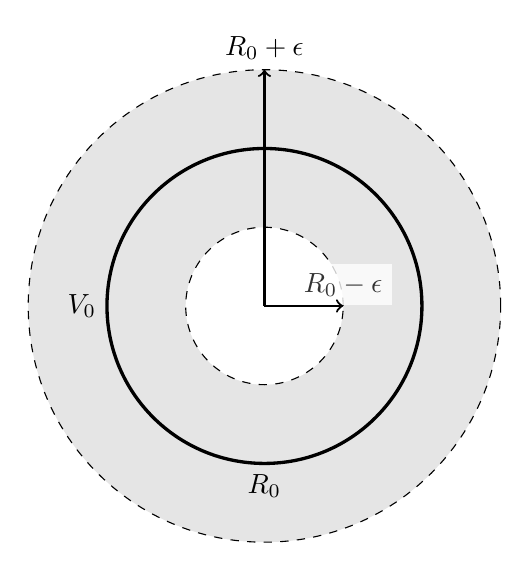
\begin{tikzpicture}[scale=1]
  \def\radiusZero{2cm}
  \def\eps{1cm}
  \draw[dashed, fill=black!10]
    (0,0) circle [radius=\radiusZero+\eps]
    ++ (0,\radiusZero+\eps) node (GPlus) [above] {$R_{0} + \epsilon$}
  ;
  \draw[dashed, fill=white]
    (0,0) circle [radius=\radiusZero-\eps]
    ++ (\radiusZero-\eps,0) node (GMinus) [right] {}
    node [above, rotate=-0, fill=white, opacity=0.8] {$R_{0} - \epsilon$}
  ;
  \draw[->, thick] (0,0) -- (GPlus);
  \draw[->, thick] (0,0) -- (GMinus);
  \draw[very thick]
    (0,0) circle [radius=\radiusZero]
    ++ (0,-\radiusZero) node (R0) [below] {$R_0$}
    (0,0) ++ (-\radiusZero,0) node  [left] {$V_0$}
  ;
\end{tikzpicture}

